\documentclass{article}

\usepackage[paperwidth=8.5in,paperheight=11in,left=1.4in,
right=1in,top=1.3in, bottom=1.4in]{geometry}
\usepackage{sectsty, tikz, color, pgfplots}
\usetikzlibrary{shapes,arrows}
\usetikzlibrary{fit}
\makeatletter
\tikzset{
  fn/.style={
    inner sep=0pt,
    fill=none,
    draw=none,
    reset transform,
    fit={(\pgf@pathminx,\pgf@pathminy) (\pgf@pathmaxx,\pgf@pathmaxy)},
  },
  reset transform/.code={\pgftransformreset}
}
\makeatother

    \usetikzlibrary{patterns}
    \tikzset{%
        dotsfill/.style={draw,pattern=dots},
    }

\pgfdeclarepatternformonly[\StripesSize]{MyStripes}{\pgfqpoint{-1pt}{-1pt}}{\pgfqpoint{4pt}{4pt}}{\pgfqpoint{\StripesSize}{\StripesSize}}%
{
  \pgfsetlinewidth{0.3pt}
  \pgfpathmoveto{\pgfqpoint{0pt}{0pt}}
  \pgfpathlineto{\pgfqpoint{3.1pt}{3.1pt}}
  \pgfusepath{stroke}
}

\newdimen\StripesSize
\tikzset{
    StripesSize/.code={\StripesSize=#1},
    StripesSize=3pt
}

\begin{document}

\begin{figure}
  \centering
    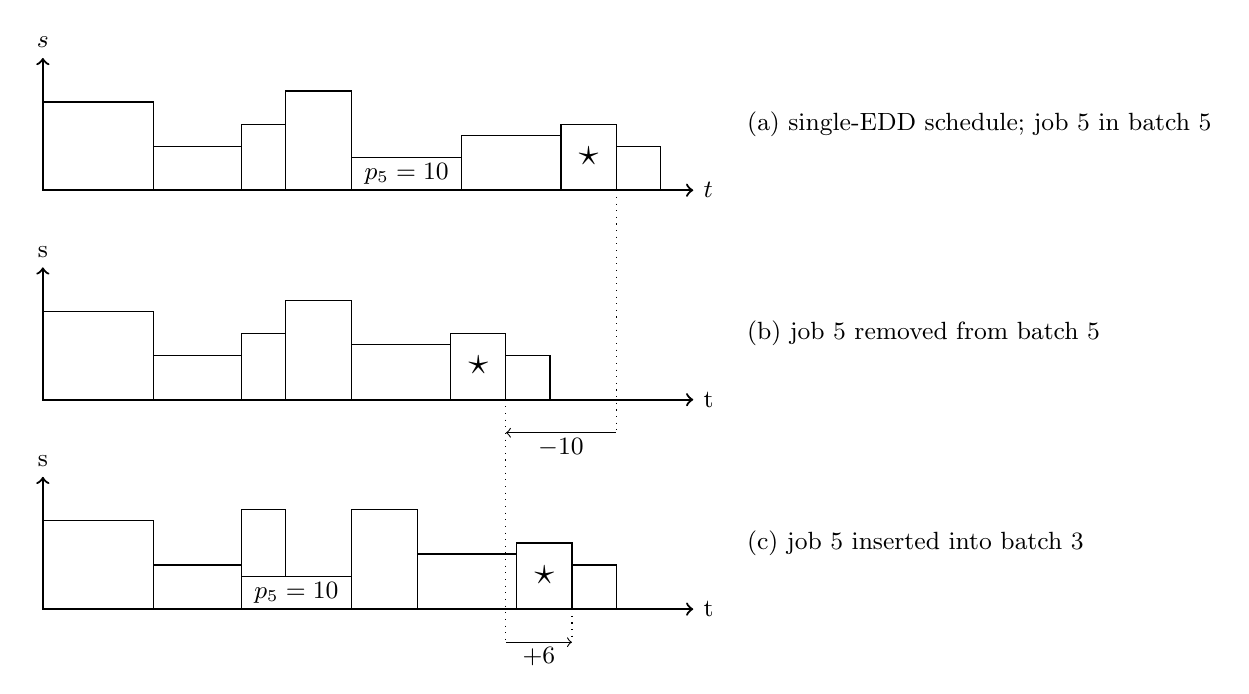
\begin{tikzpicture}[scale=0.14, font=\small]
    \draw [<->,thick] (0,12) node (yaxis) [above] {$s$}
        |- (59,0) node (xaxis) [right] {$t$};
        \draw (0,0) rectangle (10,8) ;
        \draw (10,0) rectangle (18,4) ;
        \draw (18,0) rectangle (22,6) ;
        \draw (22,0) rectangle (28,9) ;
        \draw (28,0) rectangle (38,3) node[fn,yshift=-3pt] {$p_5 = 10$};
        \draw (38,0) rectangle (47,5) ;
        \draw (47,0) rectangle (52,6) node[fn,yshift=-3pt] {\Large$\star$};
        \draw (52,0) rectangle (56,4) ;
     
      \draw[dotted] (52,0) -- (52,-22); 
    \node[anchor=west] at (63,6) {\small (a) single-EDD schedule; job 5 in batch
    5};

  \begin{scope}[shift={(0,-19)}]
     \draw [<->,thick] (0,12) node (yaxis) [above] {s}
        |- (59,0) node (xaxis) [right] {t};
        \draw (0,0) rectangle (10,8) ;
        \draw (10,0) rectangle (18,4) ;
        \draw (18,0) rectangle (22,6) ;
        \draw (22,0) rectangle (28,9) ;
        \draw (28,0) rectangle (37,5) ;
        \draw (37,0) rectangle (42,6) node[fn,yshift=-3pt] {\Large$\star$};
        \draw (42,0) rectangle (46,4) ;

    \node[anchor=west] at (63,6) {\small (b) job 5 removed from batch 5};
        \draw[dotted] (42,0) -- (42, -22);
        \draw[<-] (42,-3) -- (52,-3) node[fn, yshift=-8pt] {$-10$};
  \end{scope}

  \begin{scope}[shift={(0,-38)}]
     \draw [<->,thick] (0,12) node (yaxis) [above] {s}
        |- (59,0) node (xaxis) [right] {t};
        \draw (0,0) rectangle (10,8) ;
        \draw (10,0) rectangle (18,4) ;
        \draw (18,3) rectangle (22,9) ;
        \draw (18,0) rectangle (28,3) node[fn,yshift=-3pt] {$p_5 = 10$} ;
        \draw (28,0) rectangle (34,9) ;
        \draw (34,0) rectangle (43,5) ;
        \draw (43,0) rectangle (48,6) node[fn,yshift=-3pt] {\Large$\star$};
        \draw (48,0) rectangle (52,4) ;

    \node[anchor=west] at (63,6) {\small (c) job 5 inserted into batch 3};
        \draw[dotted] (48,0) -- (48, -3);
        \draw[->] (42,-3) -- (48,-3) node[fn, yshift=-8pt] {$+6$};
  \end{scope}

        
    \end{tikzpicture}
\end{figure}
\end{document}
